\documentclass[tikz,border=0pt]{standalone}
\usepackage{amsmath,amssymb}
\usepackage{lmodern}
\DeclareMathSizes{10}{10}{7}{7}
\DeclareMathSizes{8}{8}{7}{7}
\usetikzlibrary{arrows.meta,shapes.geometric}
\definecolor{leftline}{RGB}{45,153,219}
\definecolor{leftfill}{RGB}{235,246,255}
\definecolor{midline}{RGB}{78,194,91}
\definecolor{midfill}{RGB}{236,250,236}
\definecolor{rightline}{RGB}{243,151,49}
\definecolor{rightfill}{RGB}{255,243,230}
\definecolor{trainline}{RGB}{137,84,198}
\definecolor{trainfill}{RGB}{249,243,255}
\definecolor{softblue}{RGB}{226,239,254}
\definecolor{softviolet}{RGB}{244,238,254}
\definecolor{softgreen}{RGB}{225,244,225}
\definecolor{softred}{RGB}{255,229,229}
\newcommand{\tinyfig}{\fontsize{9.1}{10.5}\selectfont}
\newcommand{\smallfig}{\fontsize{9.1}{10.5}\selectfont}
\newcommand{\headfig}{\fontsize{9.1}{10.5}\selectfont\bfseries}
\newcommand{\mathfig}{\fontsize{10}{11.5}\selectfont}
\begin{document}
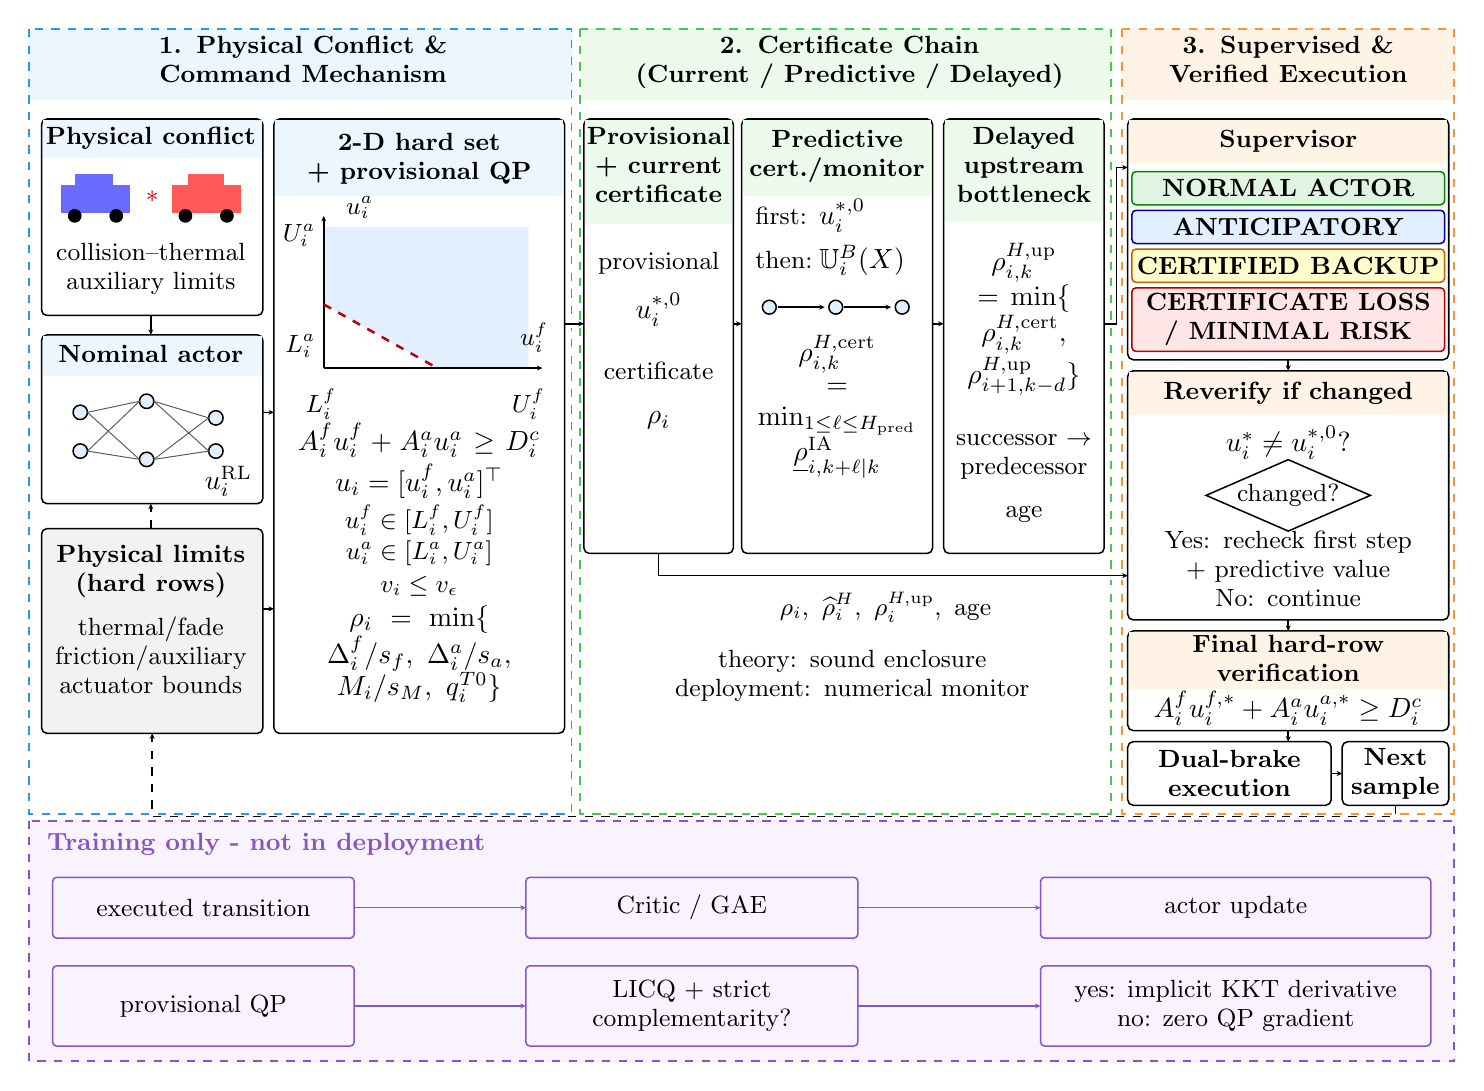
\begin{tikzpicture}[x=1pt,y=-1pt,line width=.55pt,
  mainflow/.style={draw=black,line width=.55pt,-{Stealth[length=2pt,width=1.8pt]}},
  trainingflow/.style={draw=trainline,line width=.45pt,-{Stealth[length=2pt,width=1.8pt]}},
  every node/.style={inner sep=0pt,outer sep=0pt}]
  % Fixed 516-pt print canvas. No global scale is used at integration width.
  \path[use as bounding box] (0,0) rectangle (516,374);
  \fill[leftfill] (0,0) rectangle (197,26);
  \fill[midfill] (200,0) rectangle (392,26);
  \fill[rightfill] (395,0) rectangle (516,26);
  \draw[leftline,dashed,line width=.7pt] (.5,.5) rectangle (196.5,284);
  \draw[midline,dashed,line width=.7pt] (199.5,.5) rectangle (391.5,284);
  \draw[rightline,dashed,line width=.7pt] (395.5,.5) rectangle (515.5,284);
  % Small white gateways keep signal arrows visually separate from dashed grouping borders.
  \fill[white] (195.7,105.5) rectangle (197.3,108.5);
  \fill[white] (198.7,105.5) rectangle (200.3,108.5);
  \fill[white] (390.7,105.5) rectangle (392.3,108.5);
  \fill[white] (394.7,49) rectangle (396.3,52);
  \fill[white] (390.7,196.5) rectangle (392.3,199.5);
  \fill[white] (394.7,196.5) rectangle (396.3,199.5);
  \fill[white] (493.25,283.3) rectangle (495.25,284.7);
  \fill[white] (44,283.3) rectangle (46,284.7);
  \node[anchor=north,align=center,font=\headfig,text width=190pt] at (99.5,3) {1. Physical Conflict \&\\Command Mechanism};
  \node[anchor=north,align=center,font=\headfig,text width=184pt] at (297,3) {2. Certificate Chain\\(Current / Predictive / Delayed)};
  \node[anchor=north,align=center,font=\headfig,text width=116pt] at (455.5,3) {3. Supervised \&\\Verified Execution};

  % Section 1: opposed physics, nominal proposal, hard geometry and exact reserve.
  \draw[rounded corners=2pt] (5,33) rectangle (85,104);
  \fill[leftfill] (5.5,33.5) rectangle (84.5,47);
  \node[font=\smallfig\bfseries] at (44.5,40) {Physical conflict};
  \fill[blue!58] (12,57) rectangle (37,67);
  \fill[blue!58] (17,53) rectangle (31,58);
  \draw[fill=black] (17,68) circle (2.2);
  \draw[fill=black] (32,68) circle (2.2);
  \fill[red!65] (52,57) rectangle (77,67);
  \fill[red!65] (58,53) rectangle (71,58);
  \draw[fill=black] (57,68) circle (2.2);
  \draw[fill=black] (72,68) circle (2.2);
  \node[font=\headfig,text=red!80!black] at (45,61) {$\ast$};
  \node[anchor=north,align=center,font=\tinyfig,text width=77pt] at (44.5,78) {collision--thermal\\auxiliary limits};

  \draw[rounded corners=2pt] (5,111) rectangle (85,172);
  \fill[leftfill] (5.5,111.5) rectangle (84.5,126);
  \node[font=\smallfig\bfseries] at (44.5,118) {Nominal actor};
  \foreach \p in {(19,139),(19,153),(43,135),(43,156),(68,141),(68,153)} {\draw[fill=softblue] \p circle (2.6);}
  \foreach \ya in {139,153} {\foreach \yb in {135,156} {\draw[black!65,line width=.35pt] (21.6,\ya) -- (40.4,\yb);}}
  \foreach \ya in {135,156} {\foreach \yb in {141,153} {\draw[black!65,line width=.35pt] (45.6,\ya) -- (65.4,\yb);}}
  \node[font=\mathfig,anchor=east] at (81,164) {$u_i^{\rm RL}$};

  \draw[rounded corners=2pt,fill=black!5] (5,181) rectangle (85,255);
  \node[anchor=north,align=center,font=\smallfig\bfseries,text width=73pt] at (44.5,187) {Physical limits\\(hard rows)};
  \node[anchor=north,align=center,font=\tinyfig,text width=76pt] at (44.5,213) {thermal/fade\\friction/auxiliary\\actuator bounds};
  \draw[mainflow] (44.5,104) -- (44.5,111);
  \draw[mainflow,dashed] (44.5,181) -- (44.5,172);

  \draw[rounded corners=2pt] (89,33) rectangle (194,255);
  \fill[leftfill] (89.5,33.5) rectangle (193.5,61);
  \node[anchor=north,align=center,font=\smallfig\bfseries,text width=101pt] at (141.5,38) {2-D hard set\\+ provisional QP};
  \draw[mainflow] (85,139) -- (89,139);
  \draw[mainflow] (85,210) -- (89,210);
  % Correct northeast side of the coupled collision face is shaded.
  \fill[softblue] (107,72) -- (181,72) -- (181,123) -- (148,123) -- (107,100) -- cycle;
  \draw[mainflow] (107,123) -- (186,123);
  \draw[mainflow] (107,123) -- (107,68);
  \draw[red!75!black,dashed,line width=.9pt] (107,100) -- (148,123);
  \node[font=\tinyfig] at (106,136) {$L_i^f$};
  \node[font=\tinyfig] at (181,136) {$U_i^f$};
  \node[font=\tinyfig,anchor=east] at (104,75) {$U_i^a$};
  \node[font=\tinyfig,anchor=east] at (104,115) {$L_i^a$};
  \node[font=\smallfig] at (183,112) {$u_i^f$};
  \node[font=\smallfig] at (120,65) {$u_i^a$};
  \node[anchor=north,align=center,font=\mathfig,text width=102pt] at (141.5,143) {$A_i^fu_i^f+A_i^au_i^a\ge D_i^c$};
  \node[font=\mathfig] at (141.5,164) {$u_i=[u_i^f,u_i^a]^\top$};
  \node[font=\smallfig] at (141.5,178) {$u_i^f\in[L_i^f,U_i^f]$};
  \node[font=\smallfig] at (141.5,190) {$u_i^a\in[L_i^a,U_i^a]$};
  \node[font=\smallfig] at (141.5,202) {$v_i\le v_\epsilon$};
  \node[anchor=north,align=center,font=\mathfig,text width=101pt] at (141.5,209) {$\rho_i=\min\{$\\$\Delta_i^f/s_f,\ \Delta_i^a/s_a,$\\$M_i/s_M,\ q_i^{T0}\}$};

  % Section 2: the current two-output status and finite-horizon chain.
  \draw[rounded corners=2pt] (201,33) rectangle (255,190);
  \fill[midfill] (201.5,33.5) rectangle (254.5,71);
  \node[anchor=north,align=center,font=\tinyfig\bfseries,text width=53pt] at (228,36) {Provisional\\+ current\\certificate};
  \node[font=\tinyfig] at (228,85) {provisional};
  \node[font=\mathfig] at (228,102) {$u_i^{*,0}$};
  \node[font=\tinyfig] at (228,124) {certificate};
  \node[font=\mathfig] at (228,142) {$\rho_i$};
  \draw[mainflow] (194,107) -- (201,107);

  \draw[rounded corners=2pt] (258,33) rectangle (327,190);
  \fill[midfill] (258.5,33.5) rectangle (326.5,61);
  \node[anchor=north,align=center,font=\smallfig\bfseries,text width=66pt] at (292.5,37) {Predictive\\cert./monitor};
  \node[font=\tinyfig,anchor=west] at (263,68) {first:};
  \node[font=\mathfig,anchor=west] at (286,68) {$u_i^{*,0}$};
  \node[font=\tinyfig,anchor=west] at (263,84) {then:};
  \node[font=\mathfig,anchor=west] at (286,84) {$\mathbb U_i^B(X)$};
  \foreach \cx in {268,292,316} {\draw[fill=softblue] (\cx,101) circle (2.5);}
  \draw[mainflow] (271,101) -- (288,101);
  \draw[mainflow] (295,101) -- (312,101);
  \node[anchor=north,align=center,font=\mathfig,text width=66pt] at (292.5,111) {$\rho_{i,k}^{H,\mathrm{cert}}$\\$=\min_{1\le\ell\le H_{\rm pred}}$\\$\underline\rho_{i,k+\ell\mid k}^{\rm IA}$};
  \draw[mainflow] (255,107) -- (258,107);

  \draw[rounded corners=2pt] (331,33) rectangle (389,190);
  \fill[midfill] (331.5,33.5) rectangle (388.5,70);
  \node[anchor=north,align=center,font=\tinyfig\bfseries,text width=54pt] at (360,36) {Delayed\\upstream\\bottleneck};
  \node[anchor=north,align=center,font=\mathfig,text width=54pt] at (360,78) {$\rho_{i,k}^{H,\rm up}$\\$=\min\{$\\$\rho_{i,k}^{H,\rm cert},$\\$\rho_{i+1,k-d}^{H,\rm up}\}$};
  \node[anchor=north,align=center,font=\tinyfig,text width=54pt] at (360,147) {successor $\to$\\predecessor};
  \node[font=\smallfig] at (360,176) {age};
  \draw[mainflow] (327,107) -- (331,107);
  \draw[mainflow] (389,107) -- (393.5,107) -- (393.5,50.5) -- (397.5,50.5);
  \draw[mainflow] (228,190) -- (228,198) -- (397.5,198);
  \node[anchor=north,font=\tinyfig] at (310,204) {$\rho_i,\ \widehat{\rho}_i^H,\ \rho_i^{H,\rm up},\ \mathrm{age}$};
  \node[anchor=north,align=center,font=\smallfig,text width=173pt] at (298,225) {theory: sound enclosure\\deployment: numerical monitor};

  % Section 3: four-mode supervision, changed-action check and verified actuation.
  \draw[rounded corners=2pt] (397.5,33) rectangle (513.5,120);
  \fill[rightfill] (398,33.5) rectangle (513,49);
  \node[font=\smallfig\bfseries] at (455.5,41) {Supervisor};
  \filldraw[fill=softgreen,draw=green!55!black,rounded corners=1.5pt] (399,52) rectangle (512,64);
  \filldraw[fill=softblue,draw=blue!65!black,rounded corners=1.5pt] (399,66) rectangle (512,78);
  \filldraw[fill=yellow!20,draw=orange!75!black,rounded corners=1.5pt] (399,80) rectangle (512,92);
  \filldraw[fill=softred,draw=red!70!black,rounded corners=1.5pt] (399,94) rectangle (512,117);
  \node[font=\smallfig\bfseries] at (455.5,58) {NORMAL ACTOR};
  \node[font=\smallfig\bfseries] at (455.5,72) {ANTICIPATORY};
  \node[font=\smallfig\bfseries] at (455.5,86) {CERTIFIED BACKUP};
  \node[font=\tinyfig\bfseries,align=center] at (455.5,105.5) {CERTIFICATE LOSS\\/ MINIMAL RISK};

  \draw[rounded corners=2pt] (397.5,124) rectangle (513.5,214);
  \fill[rightfill] (398,124.5) rectangle (513,140);
  \node[font=\smallfig\bfseries] at (455.5,132) {Reverify if changed};
  \node[font=\mathfig] at (455.5,150) {$u_i^*\ne u_i^{*,0}$?};
  \node[diamond,draw,aspect=2.3,inner sep=.6pt,font=\tinyfig] at (455.5,169) {changed?};
  \node[anchor=north,align=center,font=\tinyfig,text width=110pt] at (455.5,182) {Yes: recheck first step\\+ predictive value\\No: continue};
  \draw[mainflow] (455.5,120) -- (455.5,124);
  \draw[mainflow] (455.5,214) -- (455.5,218);

  \draw[rounded corners=2pt] (397.5,218) rectangle (513.5,254);
  \fill[rightfill] (398,218.5) rectangle (513,239);
  \node[align=center,font=\tinyfig\bfseries] at (455.5,228) {Final hard-row\\verification};
  \node[font=\mathfig] at (455.5,246) {$A_i^fu_i^{f,*}+A_i^au_i^{a,*}\ge D_i^c$};
  \draw[mainflow] (455.5,254) -- (455.5,258);
  \draw[rounded corners=2pt] (397.5,258) rectangle (471,281);
  \draw[rounded corners=2pt] (475,258) rectangle (513.5,281);
  \node[align=center,font=\tinyfig\bfseries,text width=70pt] at (434.25,269.5) {Dual-brake\\execution};
  \node[align=center,font=\tinyfig\bfseries,text width=35pt] at (494.25,269.5) {Next\\sample};
  \draw[mainflow] (471,269.5) -- (475,269.5);
  \draw[mainflow,dashed] (494.25,281) -- (494.25,285) -- (45,285) -- (45,255);

  % Training is a clearly subordinate two-chain diagnostic strip.
  \fill[trainfill] (0,286) rectangle (516,374);
  \draw[trainline,dashed,line width=.7pt] (.5,286.5) rectangle (515.5,373.5);
  \node[anchor=west,font=\smallfig\bfseries,text=trainline] at (7,295) {Training only - not in deployment};
  \draw[rounded corners=1.5pt,trainline] (9,307) rectangle (118,329);
  \draw[rounded corners=1.5pt,trainline] (180,307) rectangle (300,329);
  \draw[rounded corners=1.5pt,trainline] (366,307) rectangle (507,329);
  \node[font=\smallfig] at (63.5,318) {executed transition};
  \node[font=\smallfig] at (240,318) {Critic / GAE};
  \node[font=\smallfig] at (436.5,318) {actor update};
  \draw[trainingflow] (118,318) -- (180,318);
  \draw[trainingflow] (300,318) -- (366,318);
  \draw[rounded corners=1.5pt,trainline] (9,339) rectangle (118,368);
  \draw[rounded corners=1.5pt,trainline] (180,339) rectangle (300,368);
  \draw[rounded corners=1.5pt,trainline] (366,339) rectangle (507,368);
  \node[font=\smallfig] at (63.5,353.5) {provisional QP};
  \node[font=\tinyfig,align=center] at (240,353.5) {LICQ + strict\\complementarity?};
  \node[font=\tinyfig,align=center] at (436.5,353.5) {yes: implicit KKT derivative\\no: zero QP gradient};
  \draw[trainingflow] (118,353.5) -- (180,353.5);
  \draw[trainingflow] (300,353.5) -- (366,353.5);
\end{tikzpicture}
\end{document}
